\documentclass[a4paper]{article}
\usepackage[utf8]{inputenc}
\usepackage{biblatex} %Imports biblatex package
\addbibresource{bibl.bib}
\usepackage{authblk}
\usepackage{mathtools}
\usepackage{graphicx}

\title{NNBMSS: a Novel and Fast Method for Model
Structure Selection}

\date{Summarized by, \\ Charbel Abi Hana, Adrián Garnier Artiñano \\ \textit{École Normale Supérieure Paris-Saclay} \\\medskip\today}


\author[1,2]{Amaury Lendasse}
\author[3]{Kallin Khan}
\author[3]{Edward Ratner}
\affil[1]{University of Houston - Department of Information and Logistics Technology
Houston - USA}
\affil[2]{Arcada University of Applied Sciences - Risklab
Helsinki - Finland}
\affil[3]{Edammo Inc.
Iowa City - USA}
\renewcommand\Authands{ and }
 

\begin{document}
\maketitle
\section{Introduction}
In this paper, the authors propose a novel method for model learning model selection in regression tasks. This novel method targets the process in which users tweak and fine-tune the complexity of machine learning models to obtain an optimal combination suited for the corresponding application. The computational cost, as well as manual labor that goes into such process is highlighted and is shown to be mitigated through this method by comparing to the state-of-the-art method 10-fold cross-validation (based on k-fold cross-validation). The assessment for model structure here is done by calculating the Generalization error which translates to the quantity of how well a model can predict on unseen data. Minimizing the Generalization error equates to optimally fitting the model to a dataset and avoiding underfitting (high bias) or overfitting (high variance). The main drawback of 10-fold cross validation is its computational cost and efficiency, therefore, the proposed Nearest-Neighbour Based Model Structure Selection approach (NNBMSS), according to the authors solves the computational time required by this task.

\section{Proposed Method}
The advantages of the NNBMSS method are the following:
\begin{itemize}
    \item Instead of using $ 90\% $ of the data to train the model (as it's done in 10-fold cross validation), NNBMSS uses the entire data which mitigates sampling errors.
    \item Even through NNBMSS has to search for the Nearest Neighbor for each sample in the data, it is still faster than 10-fold cross validation because the model is only built once.
\end{itemize}
The authors also present an asymptotic mathematical proof of this method; the regression model is represented by the function $f$ and the samples are $(x_i, y_i)$, sample-output of the input pair with $i \leq i \leq N$ and N is the total number of samples. $\hat{y_i}$ is the regression model output of the sample $x_i$ where $\hat{y_i} = f(x_i)$. The nearest neighbour of $x_i$ is $x_{NN(i)}$. There are two assumptions made by the authors:
\begin{itemize}
    \item $y_i$ is noisy and is not the optimal approximation of $x_i$, thus the optimal approximation of $y_i$ is $\widetilde{y_i}$ with $y_i = \widetilde{y_i} + \epsilon_i$ where $\epsilon$ is a random variable with mean zero and variance $\sigma^2$.
    \item Input space is bounded
\end{itemize}

Therefore, for $N$ tending to infinity, the nearest neighbor of a sample gets closer to the sample itself therefore
\begin{equation}
\hat{y}_{NN(i)} \underset{N\rightarrow\infty}{\rightarrow}  \hat{y_i}
\end{equation}
and,
\begin{equation}
\widetilde{y}_{NN(i)} \underset{N\rightarrow\infty}{\rightarrow}  \widetilde{y_i}
\end{equation}

The hypothesis proposed is that the metric $Var[y_i - \hat{y}_{NN(i)}]$ is a good estimator for evaluation of the optimality of a model. If the defined metric is minimized, then we can conclude that the model has fitted the data properly. The proof is divided into three cases; overfitting, underfitting and good fitting.
\begin{itemize}
    \item In a strong overfitting state, $\hat{y}_{NN(i)} \rightarrow y_{NN(i)}$, $y_i - \hat{y}_{NN(i)} = \epsilon_i - \epsilon_{NN(i)}$, therefore, $Var[y_i - \hat{y}_{NN(i)}] = 2\sigma^2$
    \item In an underfitting state, $\hat{y_i} = y_i + \alpha_i$ with $\alpha$ a random variable with zero mean and $\mu^2$ variance. As $N$ tends to infinity, $y_i - \hat{y}_{NN(i)} = \epsilon_i - \alpha_i$ and $Var[y_i - \hat{y}_{NN(i)}] = Var[\epsilon_i - \alpha_i] = \sigma^2 + \mu^2$
    \item In a good fitting state, $y_i - \hat{y}_{NN(i)} = (\widetilde{y_i}+\epsilon_i)-\widetilde{y}_{NN(i)} = \epsilon_i$ and $Var[y_i - \hat{y}_{NN)i}] = Var[\epsilon_i] = \sigma^2$
\end{itemize}

From these derivations, minimizing the estimator $Var[y_i - \hat{y}_{NN(i)}]$ is an effective strategy to choose the complexity of the regression model.
\section{Experiments and Results}

The experiments compare NNBMSS and 10-Fold Cross-Validation. The dataset used to test the validation methods was the Boston housing dataset. The main reason for utilizing this dataset was its small size witch prevents the dataset from being asymptomatic. 

% Comment about neural networks and connection
The tests are all done by using Randomized Neural Netowrks (RNNs).  This contains one layer of neurons, and the parameter that is being used to adjust grid search is the optimal value. Each method was tested and the results were averaged.



\begin{table}[!h]
    \centering
    \begin{tabular}{|c||c|c|c|}
    \hline
         Method & Test error & Comp. Time & Selected Number of Neurons  \\ \hline
         10-fold CV & $34.31 \pm 5.24$ & $1.28s$ & $56.65 \pm 35.35$  \\ \hline
         NNBMSS & $30.24 \pm 7.02$ & $0.16s$ & $104.30 \pm 21.06$ \\ \hline
    \end{tabular}
    \caption{Results indicating means and standard deviations over 100 repetitions.}
    \label{tab:results}
\end{table}

\begin{figure}[htp]
    \centering
    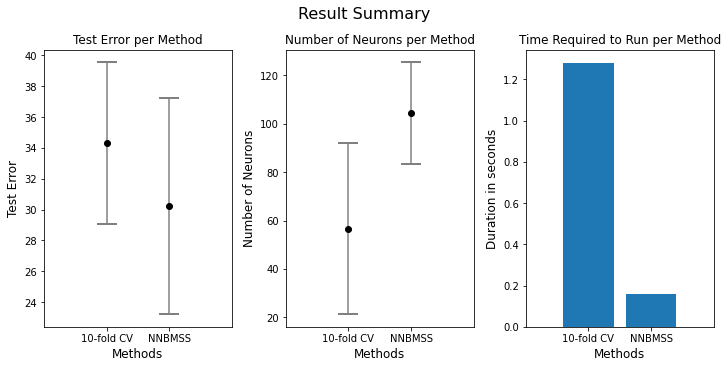
\includegraphics[width=\textwidth]{results.png}
    \caption{Summary of the results found in tests. }
    \label{fig:results}
\end{figure}

As shown in figure \ref{fig:results} both of the validation methods have similar Test Error. This indicates that the resulting models the NNBMSS picks are as good as the ones chosen by the 10-Fold cross validations. It is also shown that the time required by the NNBMSS is 8 times less than the 10-fold cross validation.

\section{Conclusion}

The NNBMSS algorithm has an efficiency of $O(N\times log(N))$. This means that it is a bit more expensive that training once a network. However, validation algorithms often require to train multiple models to verify that it is working properly, so if the models are more computational expensive like Random Forests or Deep Neural Networks, it is better to use NNBMSS to avoid training it multiple times. Additionally, NNBMSS does not require to split the data into validation and training, allowing the training of the model to have more data available, which is better in scenarios where the amount of data is small. 

\printbibliography %Prints bibliography

\end{document}
